\documentclass[a4j]{jarticle}
\usepackage[dvipdfmx]{graphicx}
\usepackage{amssymb}
\usepackage{subfigure}
\usepackage{here}

\begin{document}

\section{クラスタ数の決定}

\begin{figure}
\begin{center}
\subfigure[PseudoF]{
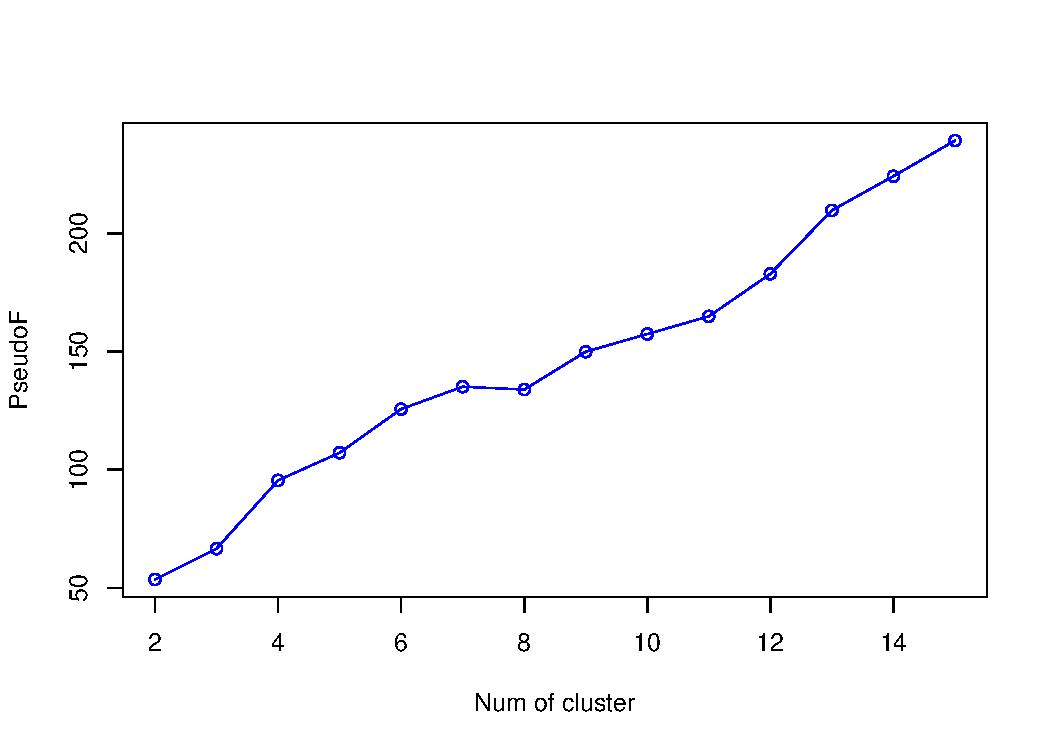
\includegraphics[height=3.5cm,width=6.5cm]{norm-PseudoF.pdf}
}~
\subfigure[主成分散布図]{
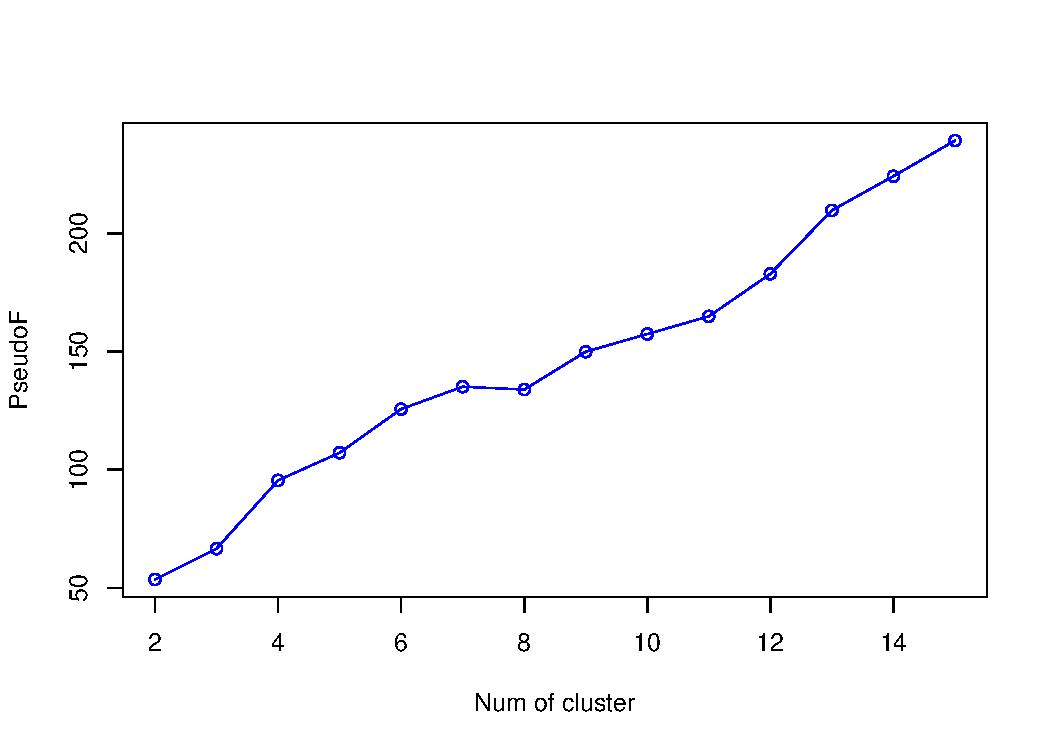
\includegraphics[height=3.5cm,width=6.5cm]{norm-PseudoF.pdf}
}\\
\subfigure[PseudoF with Mean]{
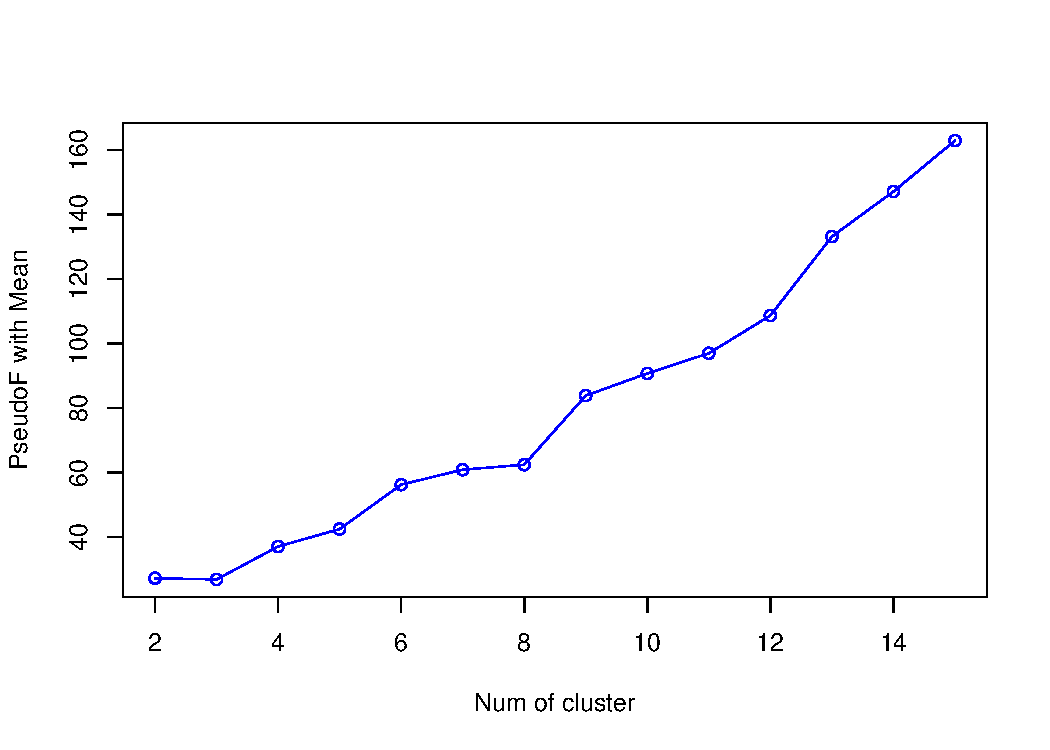
\includegraphics[height=3.5cm,width=6.5cm]{norm-PseudoFwithMean.pdf}
}~
\subfigure[主成分散布図]{
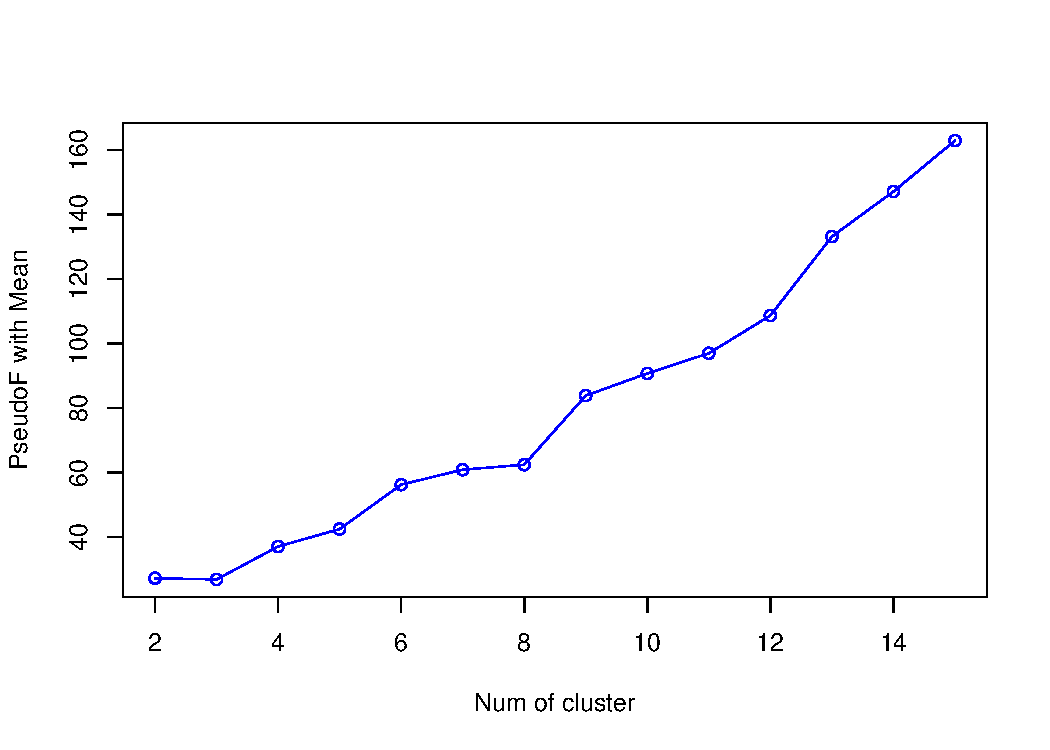
\includegraphics[height=3.5cm,width=6.5cm]{norm-PseudoFwithMean.pdf}
}\\
\subfigure[PseudoF with Min]{
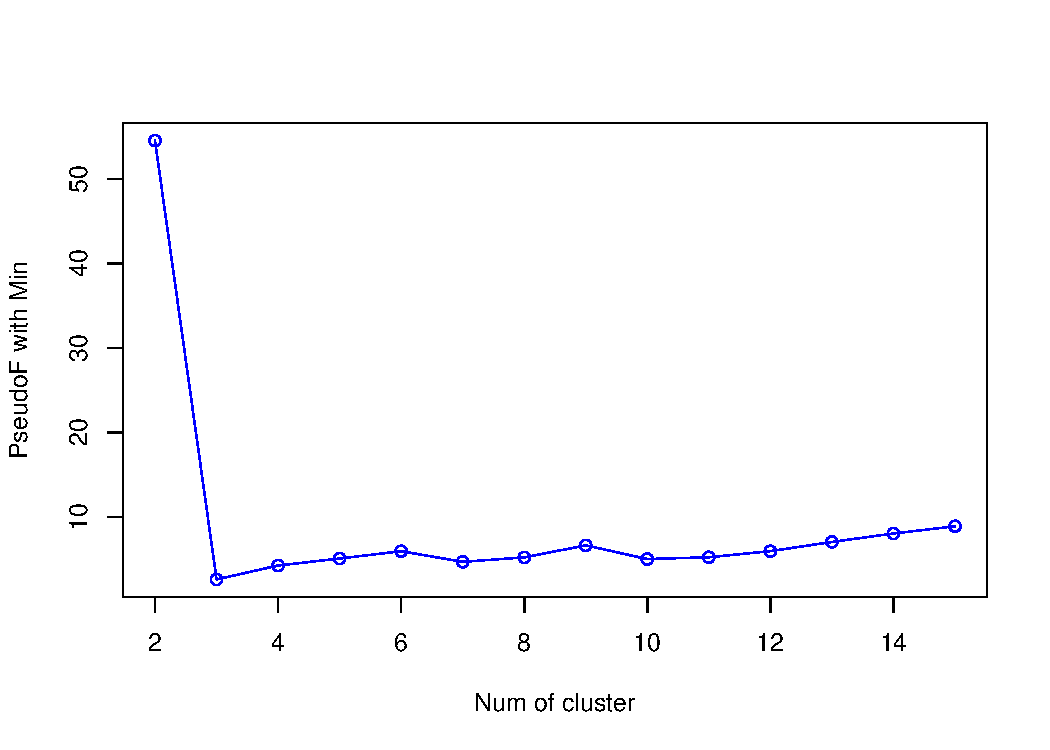
\includegraphics[height=3.5cm,width=6.5cm]{norm-PseudoFwithMin.pdf}
}~
\subfigure[主成分散布図]{
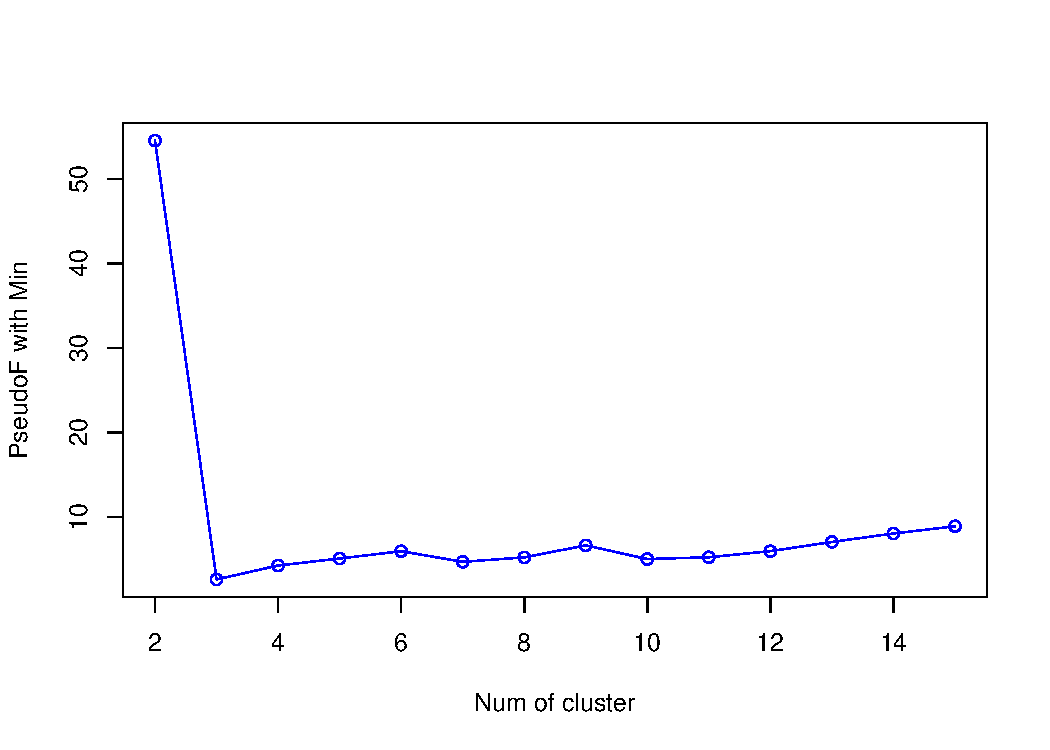
\includegraphics[height=3.5cm,width=6.5cm]{norm-PseudoFwithMin.pdf}
}\\
\caption{実測値における最適クラスタ数指標と主成分散布図}
\end{center}
\end{figure}

\begin{figure}
\begin{center}
\subfigure[PseudoF]{
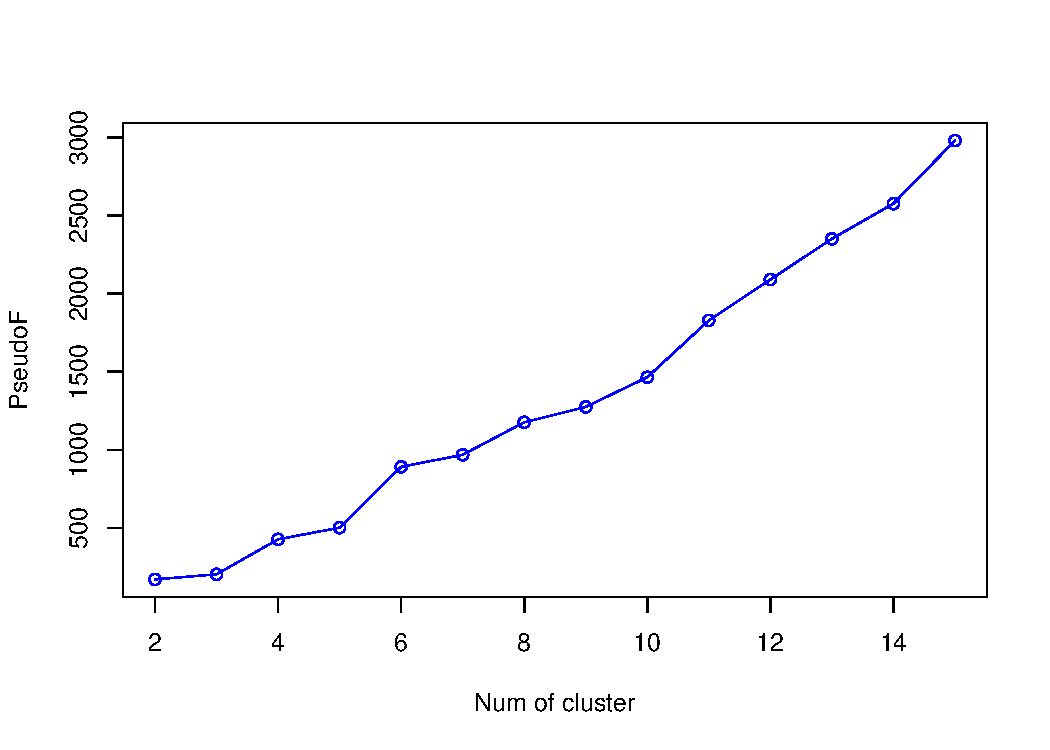
\includegraphics[height=3.5cm,width=6.5cm]{diff-PseudoF.pdf}
}~
\subfigure[主成分散布図]{
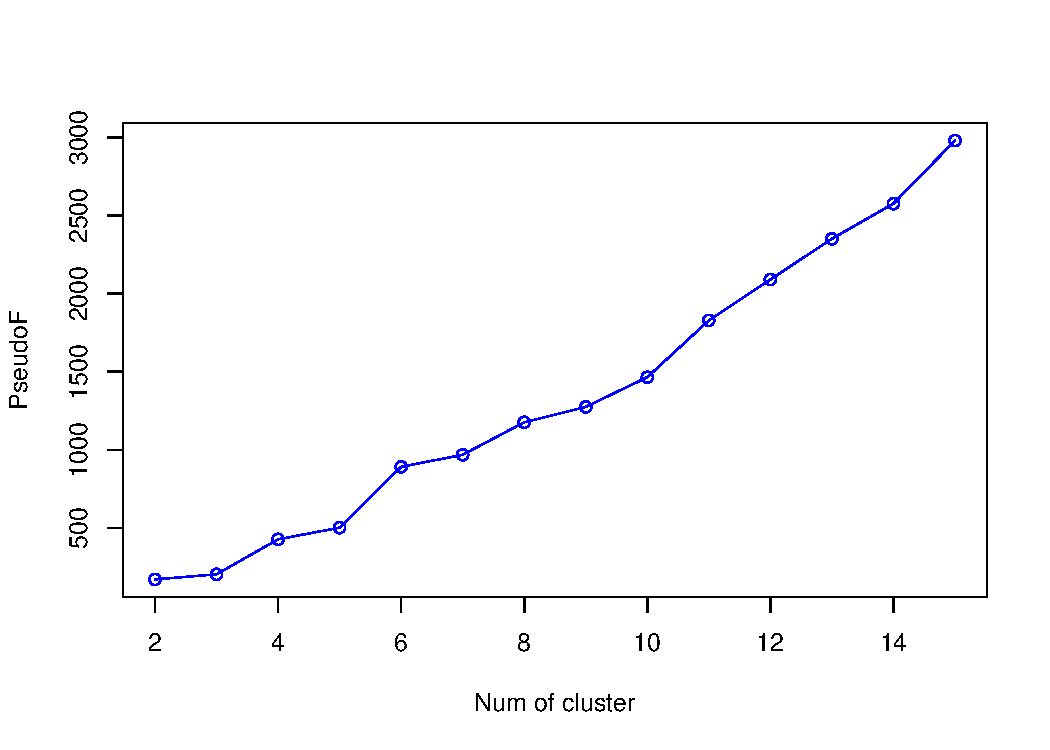
\includegraphics[height=3.5cm,width=6.5cm]{diff-PseudoF.pdf}
}\\
\subfigure[PseudoF with Mean]{
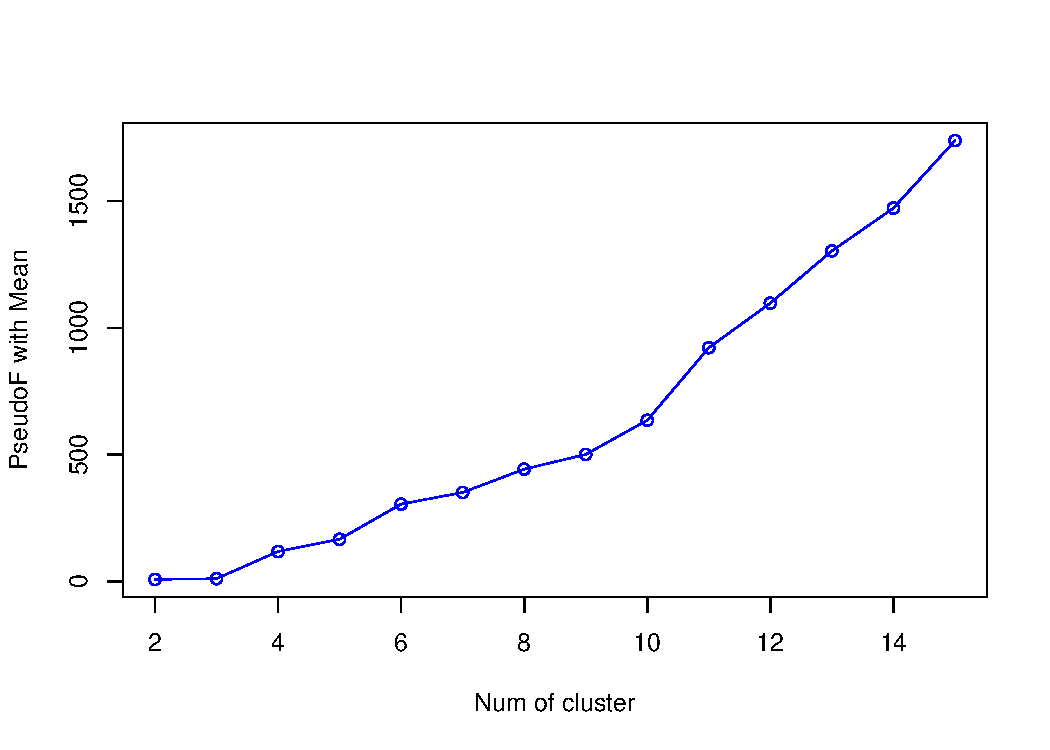
\includegraphics[height=3.5cm,width=6.5cm]{diff-PseudoFwithMean.pdf}
}~
\subfigure[主成分散布図]{
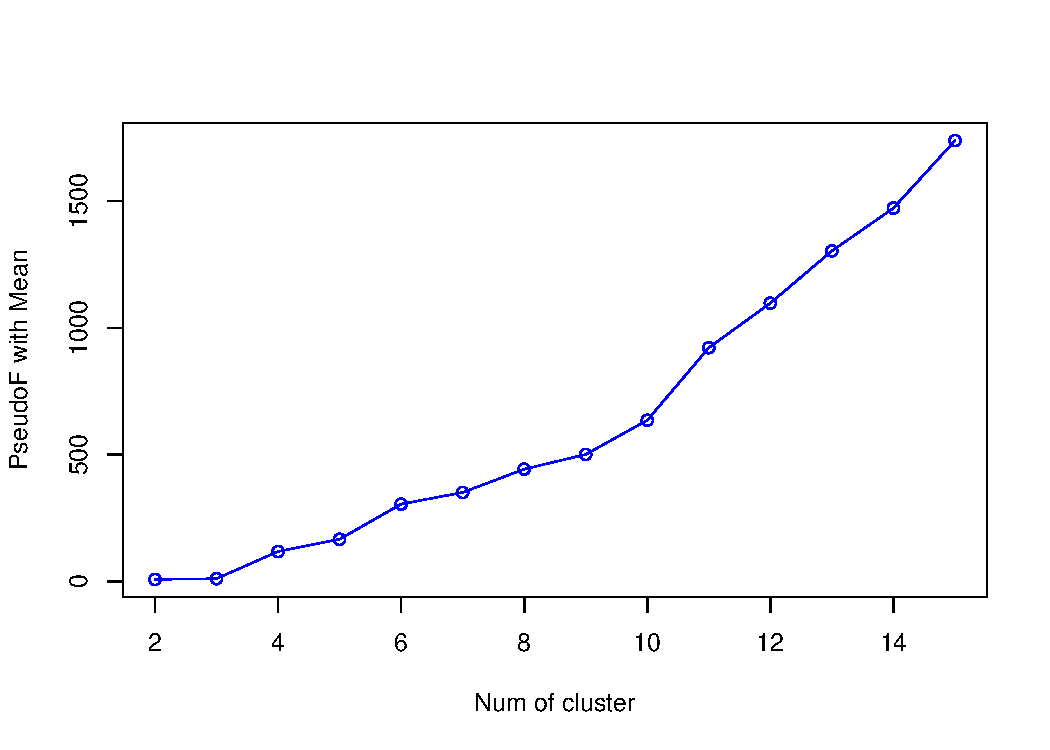
\includegraphics[height=3.5cm,width=6.5cm]{diff-PseudoFwithMean.pdf}
}\\
\subfigure[PseudoF with Min]{
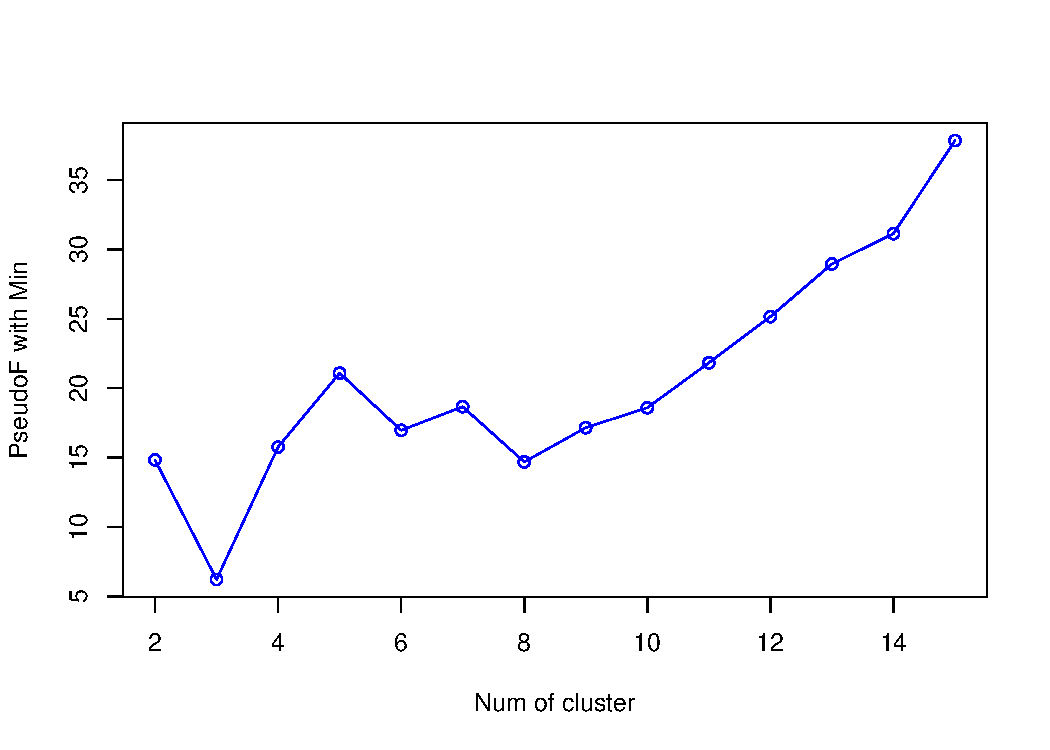
\includegraphics[height=3.5cm,width=6.5cm]{diff-PseudoFwithMin.pdf}
}~
\subfigure[主成分散布図]{
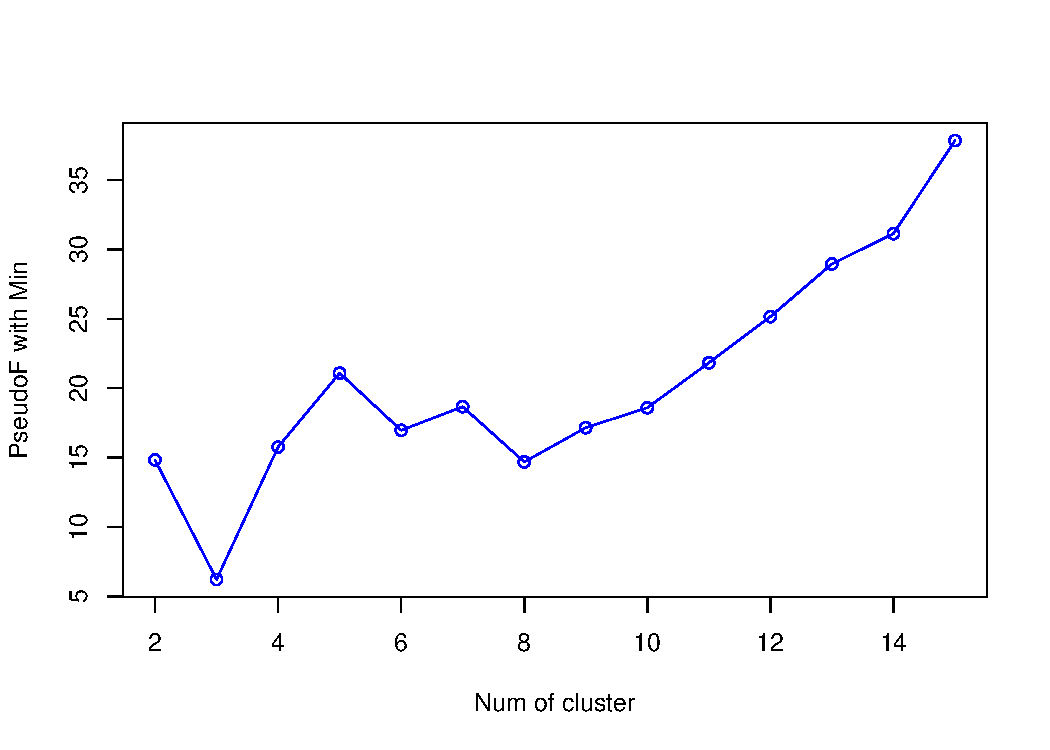
\includegraphics[height=3.5cm,width=6.5cm]{diff-PseudoFwithMin.pdf}
}\\
\caption{変動値における最適クラスタ数指標と主成分散布図}
\end{center}
\end{figure}

\begin{figure}
\begin{center}
\subfigure[PseudoF]{
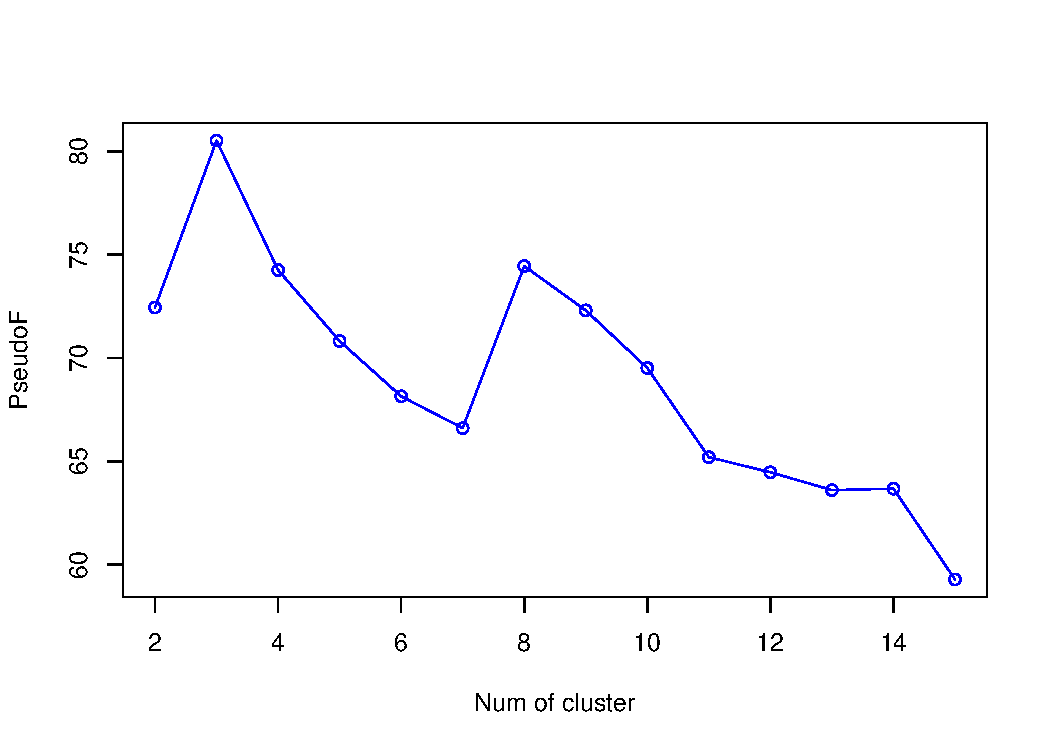
\includegraphics[height=3.5cm,width=6.5cm]{norm_comp-PseudoF.pdf}
}~
\subfigure[主成分散布図]{
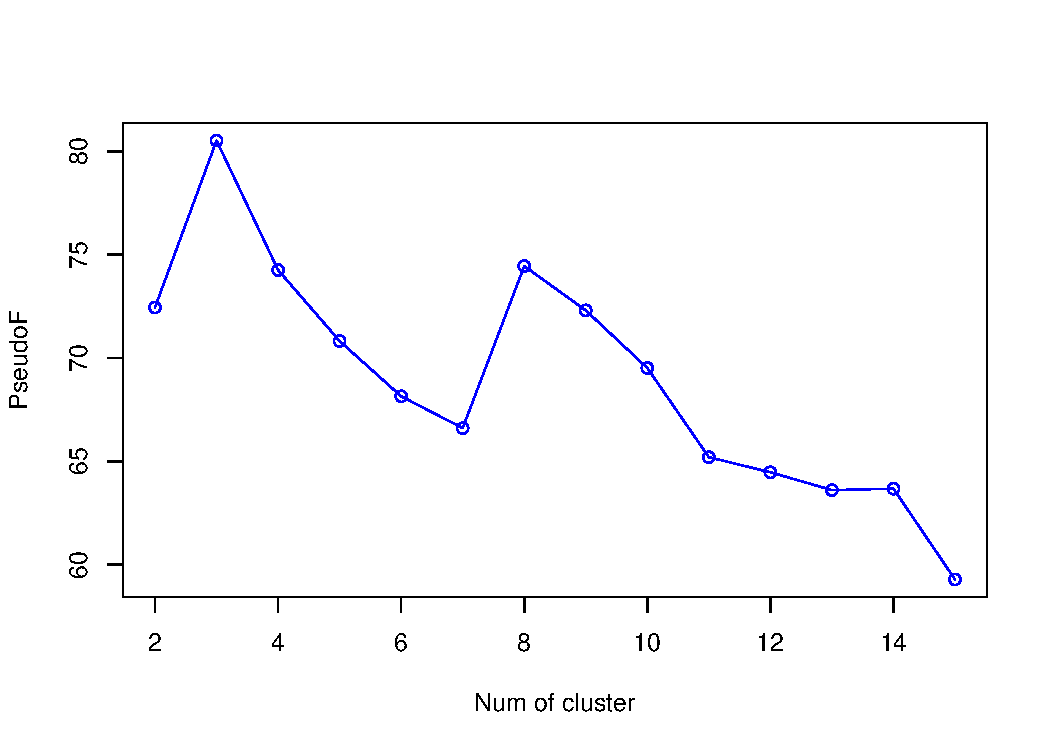
\includegraphics[height=3.5cm,width=6.5cm]{norm_comp-PseudoF.pdf}
}\\
\subfigure[PseudoF with Mean]{
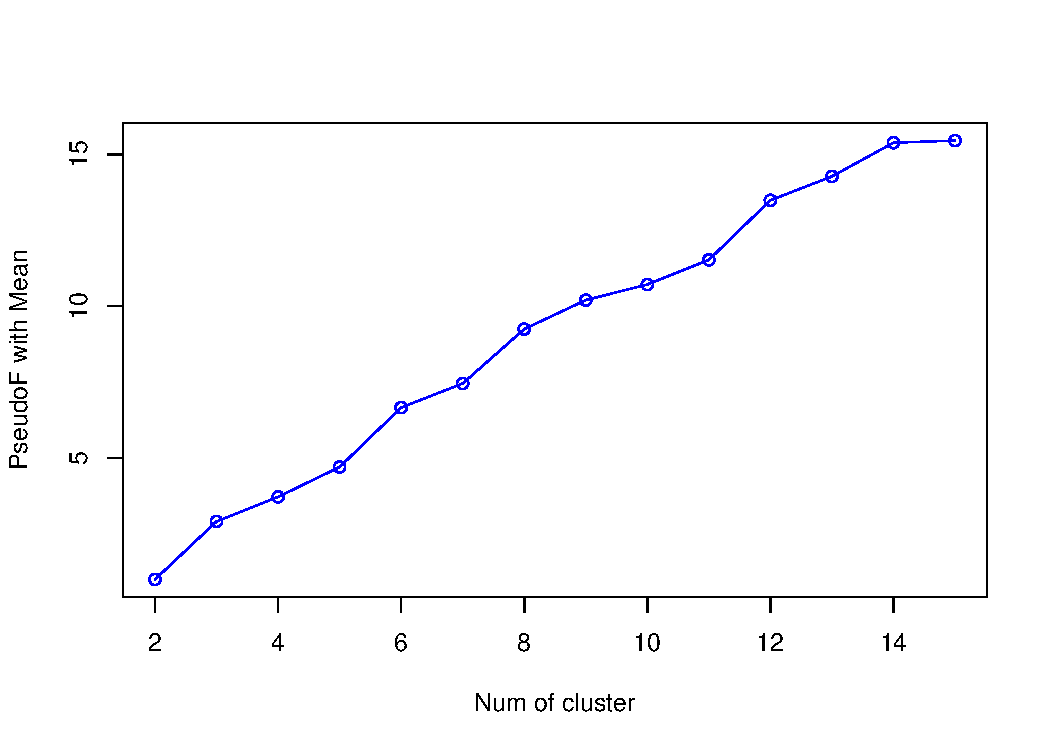
\includegraphics[height=3.5cm,width=6.5cm]{norm_comp-PseudoFwithMean.pdf}
}~
\subfigure[主成分散布図]{
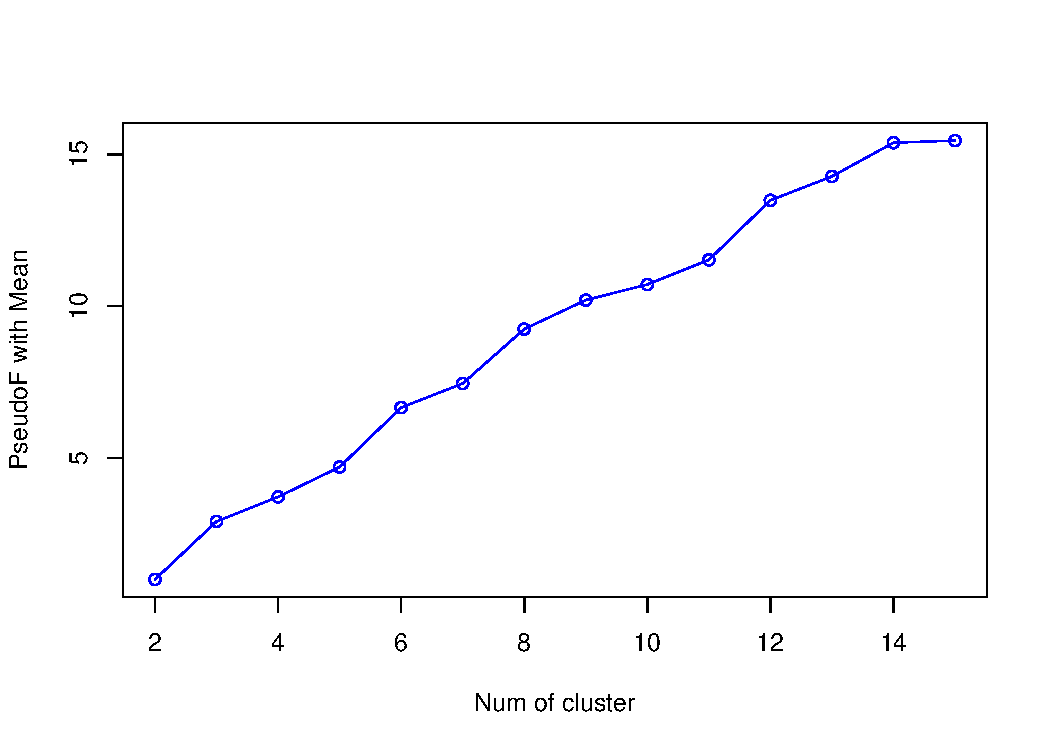
\includegraphics[height=3.5cm,width=6.5cm]{norm_comp-PseudoFwithMean.pdf}
}\\
\subfigure[PseudoF with Min]{
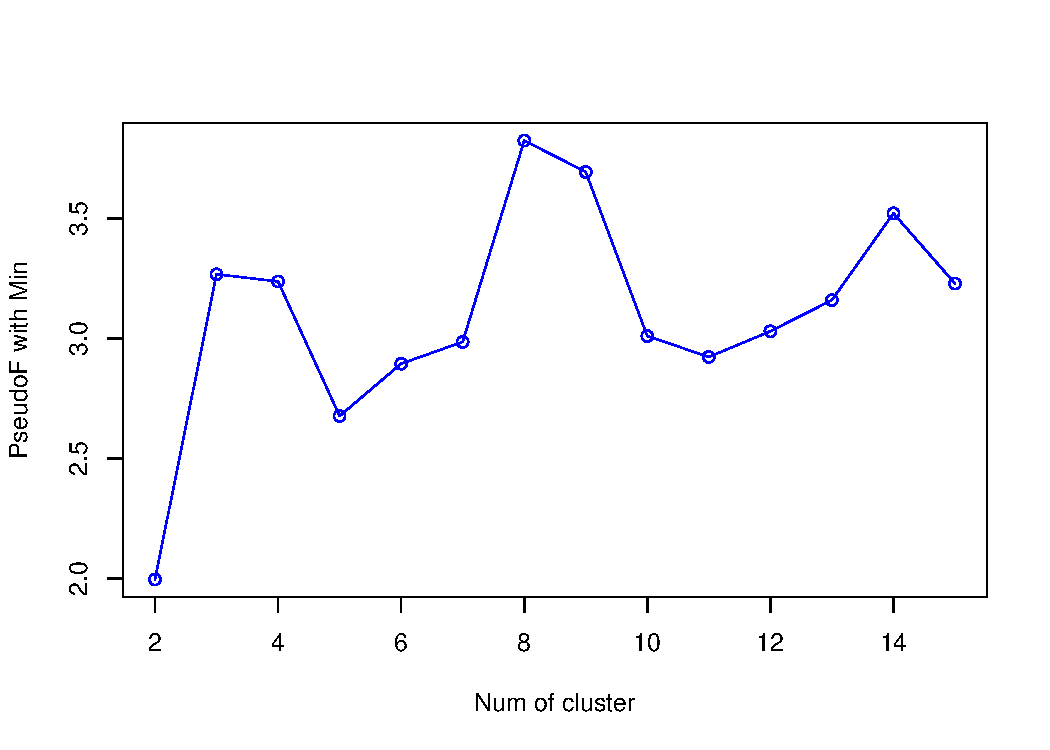
\includegraphics[height=3.5cm,width=6.5cm]{norm_comp-PseudoFwithMin.pdf}
}~
\subfigure[主成分散布図]{
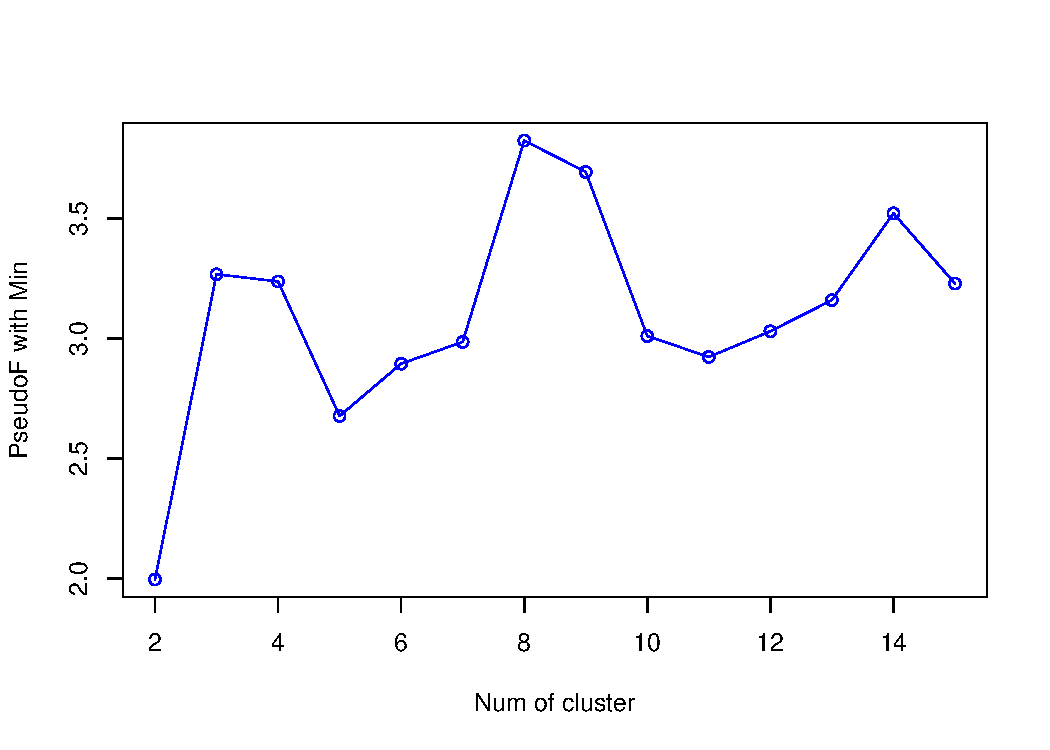
\includegraphics[height=3.5cm,width=6.5cm]{norm_comp-PseudoFwithMin.pdf}
}\\
\caption{実測値の主成分における最適クラスタ数指標と散布図}
\end{center}
\end{figure}

\begin{figure}
\begin{center}
\subfigure[PseudoF]{
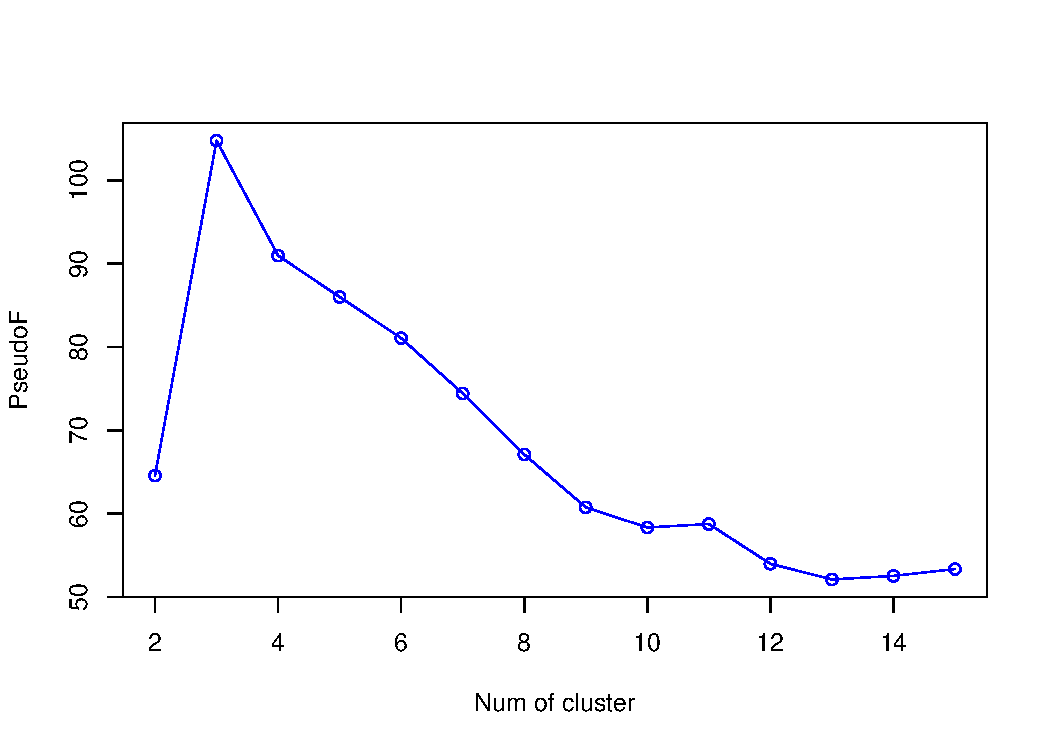
\includegraphics[height=3.5cm,width=6.5cm]{diff_comp-PseudoF.pdf}
}~
\subfigure[主成分散布図]{
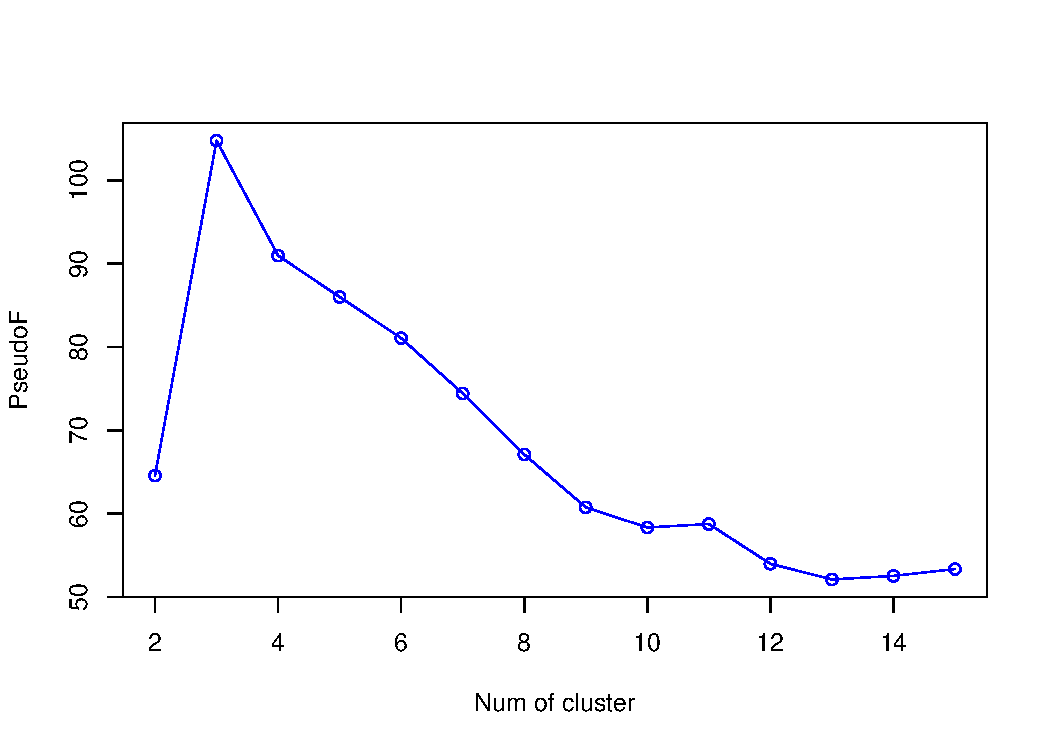
\includegraphics[height=3.5cm,width=6.5cm]{diff_comp-PseudoF.pdf}
}\\
\subfigure[PseudoF with Mean]{
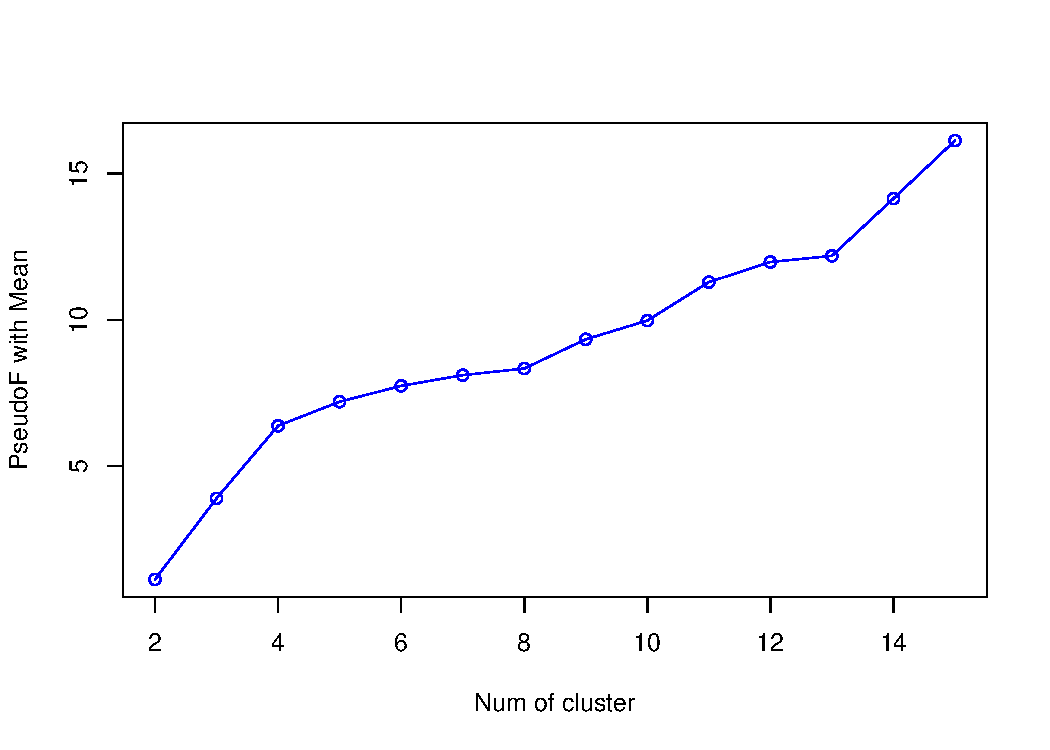
\includegraphics[height=3.5cm,width=6.5cm]{diff_comp-PseudoFwithMean.pdf}
}~
\subfigure[主成分散布図]{
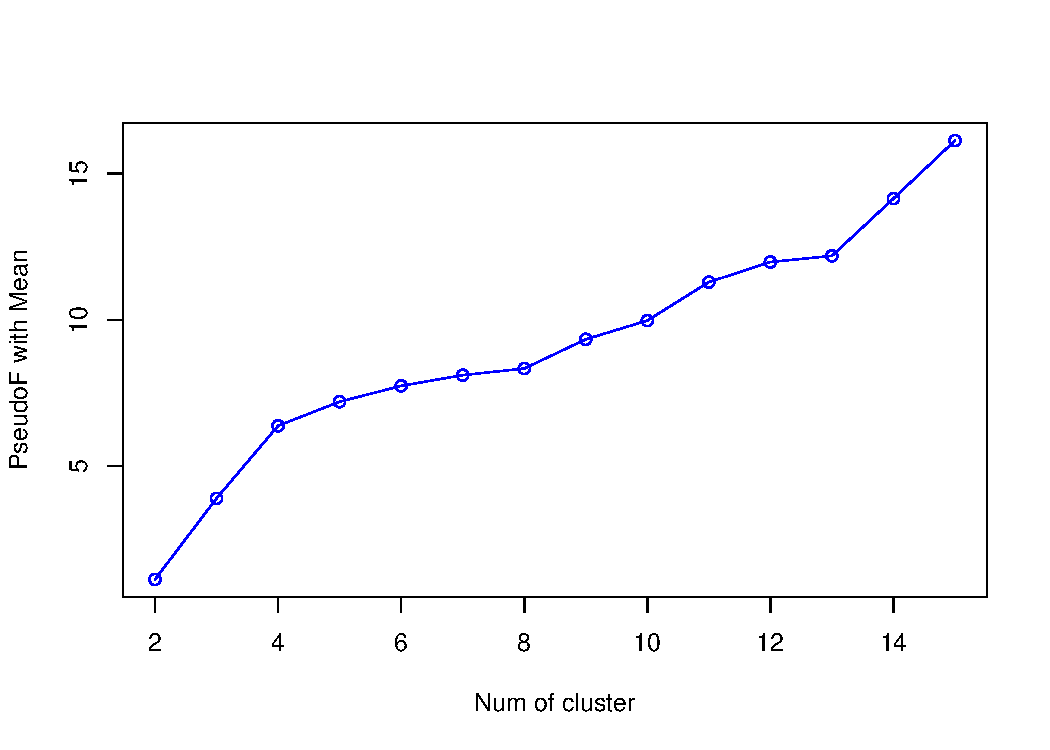
\includegraphics[height=3.5cm,width=6.5cm]{diff_comp-PseudoFwithMean.pdf}
}\\
\subfigure[PseudoF with Min]{
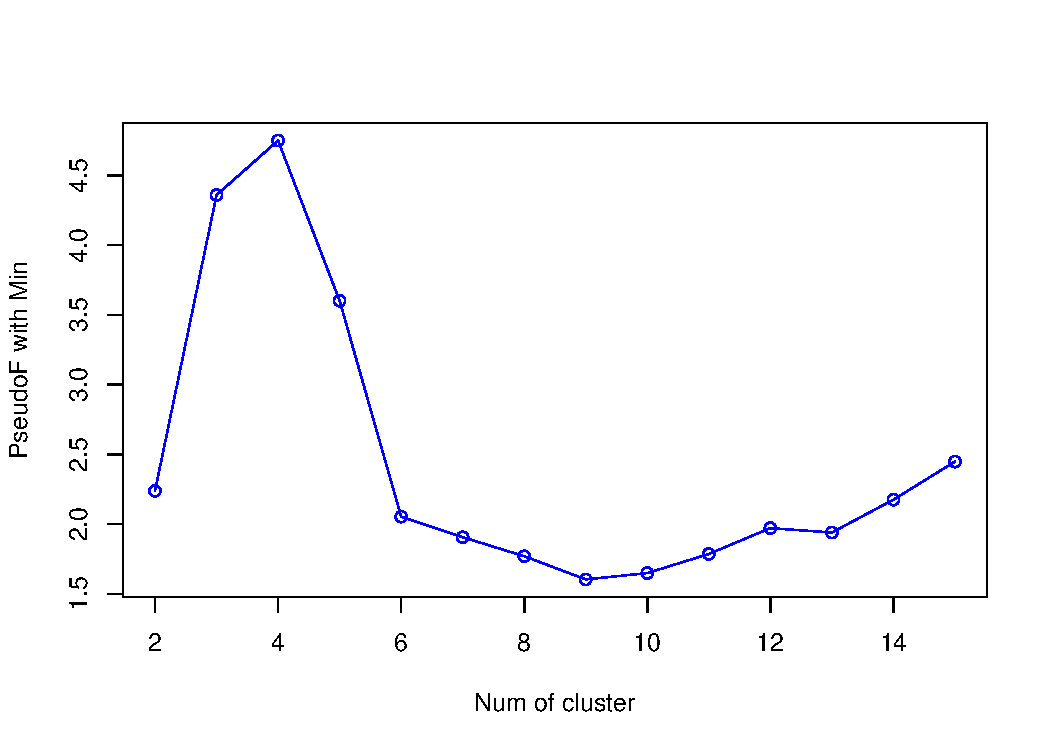
\includegraphics[height=3.5cm,width=6.5cm]{diff_comp-PseudoFwithMin.pdf}
}~
\subfigure[主成分散布図]{
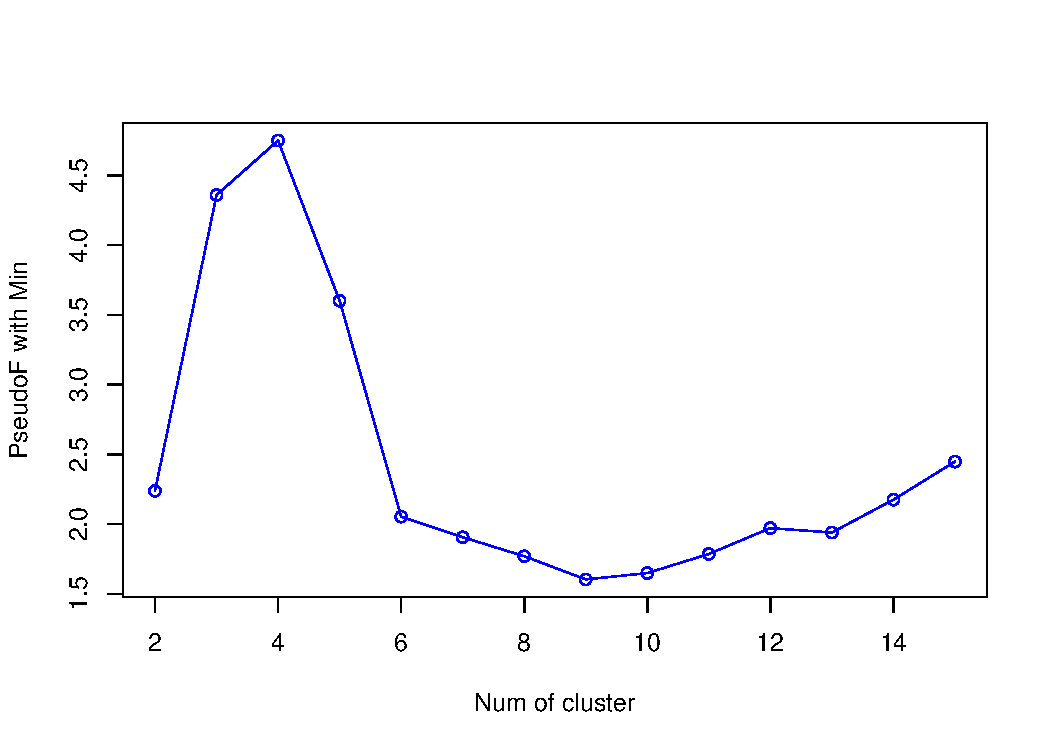
\includegraphics[height=3.5cm,width=6.5cm]{diff_comp-PseudoFwithMin.pdf}
}\\
\caption{変動値の主成分における最適クラスタ数指標と散布図}
\end{center}
\end{figure}

\end{document}